\documentclass[xcolor=table]{beamer}
\usepackage[utf8]{inputenc}
\usepackage{default}
\usepackage{xspace,setspace}
\usepackage{amsmath,amsthm,amssymb}
\usepackage{ellipsis}
\usepackage[pdftex]{epsfig}
\usepackage{listliketab}
\usepackage[table]{xcolor}
\usepackage{booktabs}

\usepackage{pgf}
\usepackage{tikz}
\usetikzlibrary{arrows,automata}
\usetikzlibrary{graphs}
\tikzset{
     mainNode/.style =
        { circle
        , draw
        %, fill=blue!20,
        %, font=\sffamily\Large\bfseries
        }
}

\usetheme{AnnArbor}
%\usetheme{Berlin}
%\usetheme{Bergen}
%\usetheme{Antibes}
%\usetheme{Goettingen}
%\usetheme{Warsaw}
%\usetheme{Darmstadt}
%\usetheme{JuanLesPins}
%\setbeamertemplate{navigation symbols}{}
%\usecolortheme{beaver}
%\usecolortheme{rose}
%\usecolortheme{seagull}
%\usecolortheme{dove}
%\usecolortheme{seahorse}
%\usecolortheme{crane}
%\usepackage{color,colortbl}
%\usepackage{texnansi}
%\usepackage{marvosym}
%\usepackage{comment}


%\setbeamertemplate{frametitle}
%{\begin{centering}\smallskip
%   \insertframetitle\par
%   \smallskip\end{centering}}
%\setbeamertemplate{itemize item}{$\bullet$}
%\setbeamertemplate{navigation symbols}{}
%\setbeamertemplate{footline}[text line]{%
%    \hfill\strut{%
%        \scriptsize\sf\color{black!60}%
%        \quad\insertframenumber
%    }%
%    \hfill
%}

% Define some colors:

\definecolor{DarkFern}{HTML}{407428}
\definecolor{DarkCharcoal}{HTML}{4D4944}
\colorlet{Fern}{DarkFern!85!white}
\colorlet{Charcoal}{DarkCharcoal!85!white}
\colorlet{LightCharcoal}{Charcoal!50!white}
\colorlet{AlertColor}{orange!80!black}
\colorlet{DarkRed}{red!70!black}
\colorlet{DarkBlue}{olive!70!black}
\colorlet{DarkGreen}{green!70!black}
\definecolor{brickred}{RGB}{132,31,39}

% Use the colors:

%\setbeamercolor{title}{fg=Fern}
%\setbeamercolor{frametitle}{fg=Fern}
%\setbeamercolor{section title}{fg=Fern}
%\setbeamercolor{section in toc}{fg=Fern}
%\setbeamercolor{section name}{fg=Fern}
%\setbeamercolor{section in head/foot}{fg=Fern}
%\setbeamercolor{subsection title}{fg=Fern}
%\setbeamercolor{author}{fg=Fern}
%\setbeamercolor{normal text}{fg=Charcoal}
%\setbeamercolor{block title}{fg=black,bg=Fern!25!white}
%\setbeamercolor{block body}{fg=black,bg=Fern!25!white}
%\setbeamercolor{alerted text}{fg=AlertColor}
%\setbeamercolor{itemize item}{fg=Charcoal}

%\definecolor{bottomcolour}{rgb}{0.32,0.3,0.38}
%\definecolor{middlecolour}{rgb}{0.08,0.08,0.16}
\definecolor{tcsyellow}{RGB}{253,255,102}
\definecolor{tcsolive}{RGB}{77,147,191}
\definecolor{tcsolivemedium}{RGB}{147,177,210}
\definecolor{tcsolivelight}{RGB}{235,239,252}

\definecolor{skyolive}{rgb}{0.2,0.6,1}
\definecolor{darkolive}{rgb}{0.1,0.1,0.6}
\definecolor{darkred}{rgb}{1,0.2,0.1}
\definecolor{darkgreen}{rgb}{0.5,0.8,0.4}
\definecolor{Olive}{rgb}{0,0.3,0}
\definecolor{seagreen}{rgb}{0.3,0.9,0.6}
\definecolor{olive}{cmyk}{0.8,0.1,0.95,0.40}
\definecolor{golden}{cmyk}{0.0,0.25,0.85,0.15}
\definecolor{darkgolden}{cmyk}{0.0,0.27,0.94,0.07}
\definecolor{orange}{cmyk}{0.0,0.35,1.0,0.07}
\definecolor{orange2}{cmyk}{0.0,0.6,1.0, 0.0}
\definecolor{pecan}{cmyk}{0.0,0.37,0.80,0.12}
\definecolor{cadmium}{cmyk}{0.0,0.40,0.93,0.00}
\definecolor{snake}{cmyk}{0.8,0.1,0.95,0.60}
\definecolor{tcsyellow}{RGB}{253,255,102}
\definecolor{tcsolive}{RGB}{77,147,191}
\definecolor{tcsolivemedium}{RGB}{147,177,210}
\definecolor{tcsolivelight}{RGB}{235,239,252}

\definecolor{LRed}{rgb}{1,.8,.8}
\definecolor{MRed}{rgb}{1,.6,.6}
\definecolor{HRed}{rgb}{1,.2,.2}

\newtheorem{defn}{Definition}
\newtheorem{asf}{ASF Inputs}
\newtheorem{claim}{Claim}

\setbeamercolor{item projected}{bg=darkred}
\setbeamertemplate{enumerate items}[orange2]
\setbeamercolor{frametitle}{fg=white,bg=orange2}
\setbeamercolor{title}{fg=white,bg=orange2}
 
\usetheme{boxes}
\setbeamertemplate{blocks}[rounded][shadow=false]
\setbeamertemplate{itemize item}{\color{orange2}$\blacktriangleright$}
\setbeamertemplate{itemize subitem}{\color{orange2}$\blacktriangleright$}
 
\setbeamercolor{block title}{use=structure,fg=brickred,bg=white}
\setbeamercolor{block body}{use=structure,fg=black,bg=white}
 

\usefonttheme{professionalfonts}
% default | professionalfonts | serif |	structurebold | structureitalicserif |structuresmallcapsserif
%\usepackage{eulervm}

%% User defined commands
\newcommand{\vect}[1]{\ensuremath{\mathbf{#1}}}
\newcommand{\calX}{\ensuremath{{\cal X}}}
\newcommand{\calY}{\ensuremath{{\cal Y}}}



\title{Machine Learning}
\begin{document}

\maketitle
\section{The Learning Problem}

\begin{frame}[t]
  \frametitle{The Essence of Machine Learning}  
\textbf{Learning from data}

  \begin{itemize}
    \item A pattern exists.
    \item There seems to be no easy mathematical relationship.
    \item We have data on it.
  \end{itemize}

\bigskip

\scriptsize{This set of slides are based on Professor Yaser 
Abu-Mostafa's course \emph{Learning from Data}. See 
\texttt{http://work.caltech.edu/telecourse.html}}
\end{frame}

\begin{frame}[t]
\frametitle{Examples of Machine Learning}
\textcolor{orange2}{\textbf{Credit Approval}}

Applicant Information:

\begin{itemize}
    \item age
    \item gender
    \item salary
    \item current debt
    \item years in job $\ldots$ 
\end{itemize}

\pause

Should we approve credit? 

\bigskip

\textbf{Data}
\begin{itemize}
    \item Data on previous applications and their credit history.
\end{itemize}
\end{frame}

\begin{frame}[t]
\frametitle{Examples of Machine Learning}
\textcolor{orange2}{\textbf{Movie Ratings}}

Predict how a user would rate a movie.

\pause

\medskip

Each user is modelled as a vector of attributes:
\begin{itemize}
    \item likes comedy?  
    \item likes block-busters?
    \item likes sci-fi?
    \item likes a specific actor?
    \item $\ldots$
\end{itemize}

\pause

How would the user rate a given movie on a scale from $1$ to $10$?

\bigskip

\textbf{Data}
\begin{itemize}
    \item Data on how other users rated the given movie. 
\end{itemize}
\end{frame}


\begin{frame}[t]
\frametitle{Components of the Learning Problem}

\textbf{Formalization}

\begin{itemize}
    \item \textbf{Input:} $\vect{x}$ (applicant information)

    \pause

    \item \textbf{Output:} $y$ (good/bad customer)
    
    \pause

    \item \textbf{Target function:} $f \colon \calX \rightarrow \calY$ (ideal credit
    approval formula)
    
    \pause

    \item \textbf{Data:} $(\vect{x}^{(1)}, y^{(1)}), \ldots, (\vect{x}^{(m)},
    y^{(m)})$ (historical records)
    
    \pause

    \item \textbf{Hypothesis:} $h \colon \calX \rightarrow \calY$ (formula to be used)
\end{itemize} 
\end{frame}

\begin{frame}[t]
\frametitle{The Learning Problem}
\begin{center}
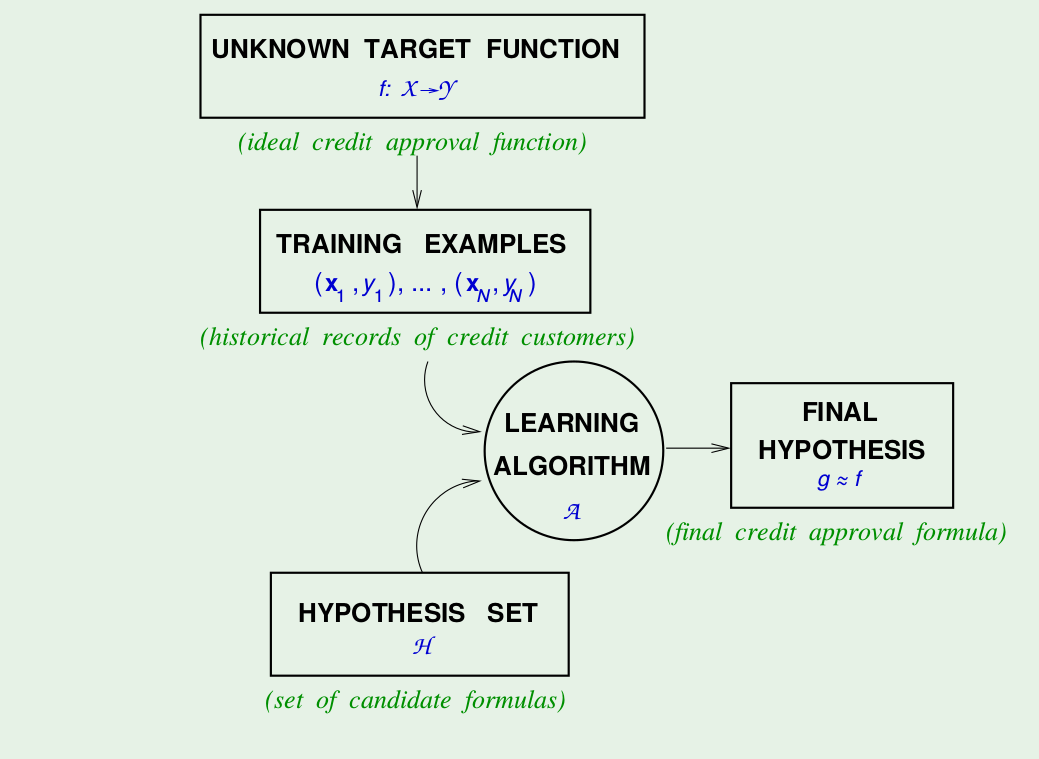
\includegraphics[scale=0.25]{the_learning_problem.png}
\end{center}
\end{frame}

\begin{frame}[t]
\frametitle{Solution Components}
Two solution components:
\begin{itemize}
    \item The Hypothesis Set $\cal{H}$
    \item The Learning Algorithm
\end{itemize}

Together, they are referred to as the \textbf{learning model}.

\pause

\bigskip

Why specify a hypothesis set?
\begin{itemize}
    \item This is what is generally done: you choose a linear model, 
    or an SVM or a neural network

    \item Important for developing a theory of learning 
\end{itemize}
\end{frame}

\begin{frame}[t]
\frametitle{Hypotheses Sets and Learning Algorithms}
\textbf{Examples}

\begin{center}
\begin{tabular}{ll}
\emph{Hypothesis Set} & \emph{Learning Algorithm} \\ \hline
Linear Regression & Gradient Descent \\
Neural Networks & Back Propagation \\
SVM & Quadratic Programming \\
Mixture of Gaussians Model & EM Algorithm \\
\end{tabular}
\end{center}
\end{frame}


\begin{frame}[t]
\frametitle{Types of Learning}
\begin{itemize}
    \item Supervised Learning
    \item Unsupervised Learning
    \item Reinforced Learning 
\end{itemize}
\end{frame}

\begin{frame}[t]
\frametitle{Supervised Learning}
\begin{center}
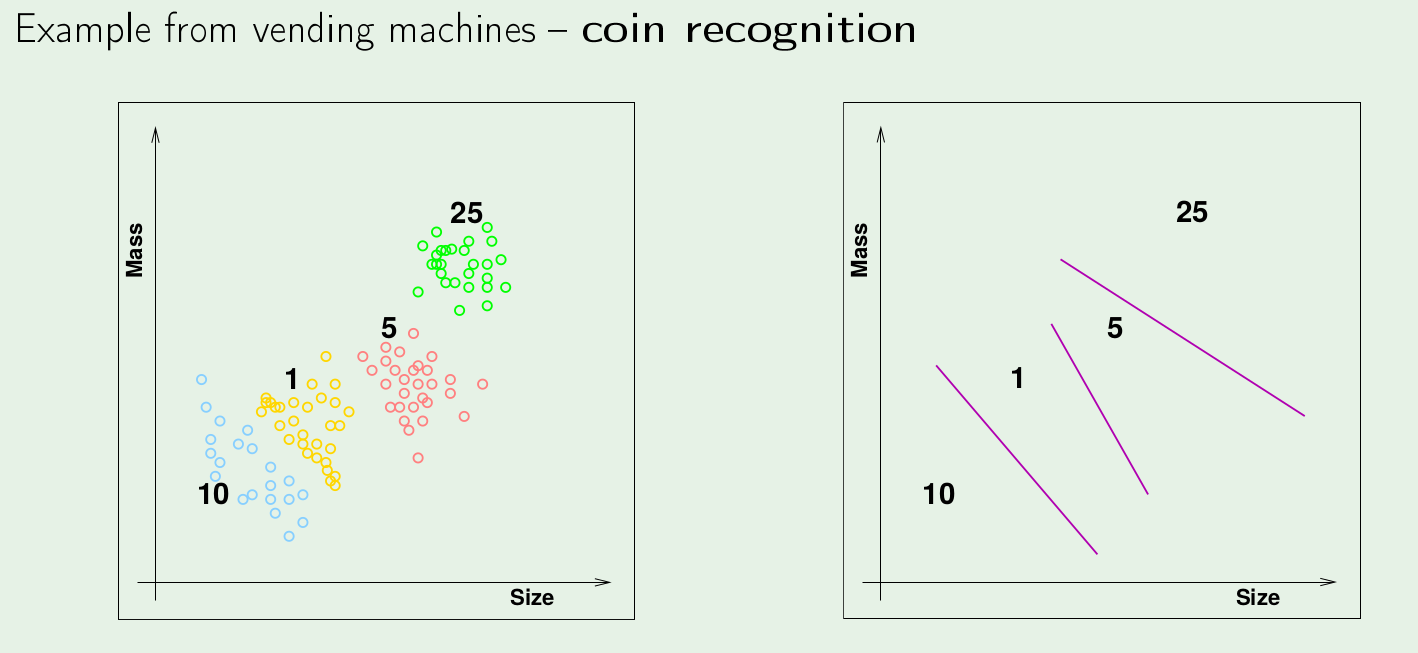
\includegraphics[scale=0.22]{supervised_learning.png}
\end{center}
\end{frame}

\begin{frame}[t]
\frametitle{Supervised Learning}
\begin{center}
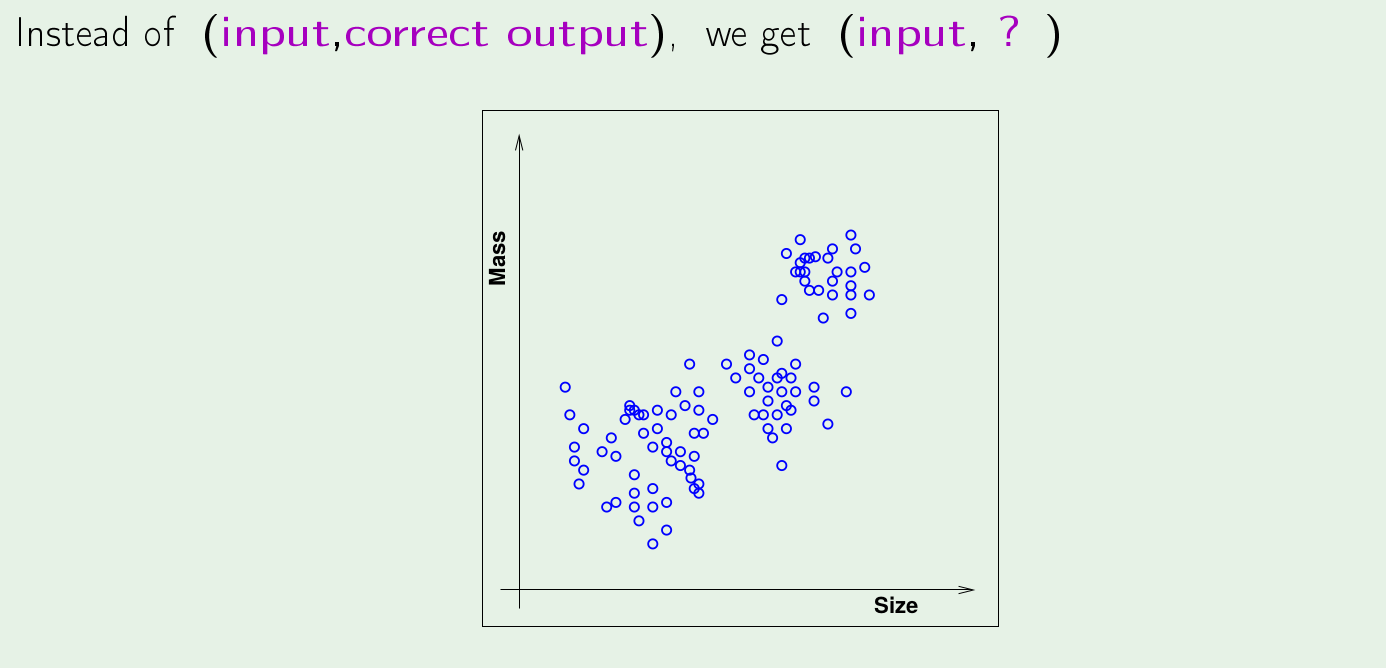
\includegraphics[scale=0.22]{unsupervised_learning.png}
\end{center}
\end{frame}

\begin{frame}[t]
\frametitle{Supervised Learning}
\begin{center}
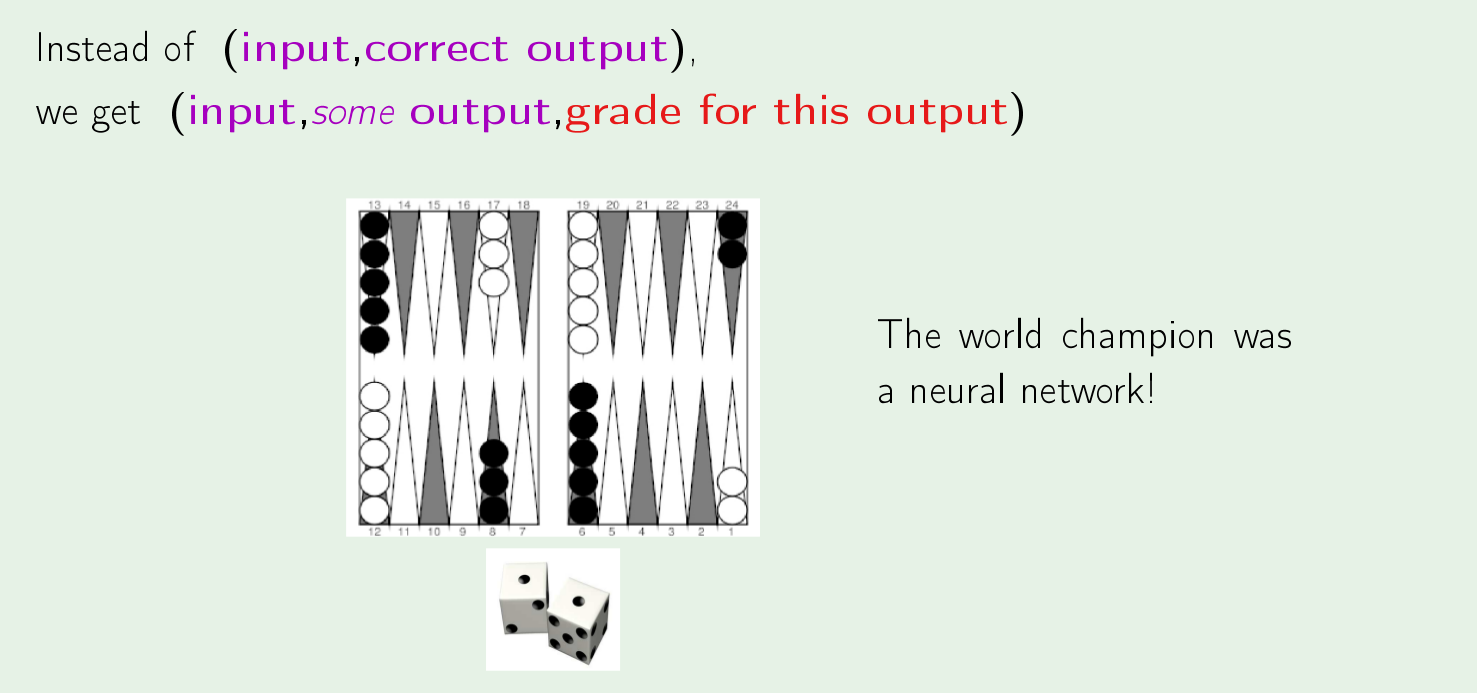
\includegraphics[scale=0.22]{reinforced_learning.png}
\end{center}
\end{frame}




\section{The Model}

\subsection{Basic Definitions}

\begin{frame}[t]
  \frametitle{Basic Definitions and Assumptions}
  \begin{definition}
  The \textcolor{orange2}{\textbf{optimisation horizon}} is a period reckoned in
  weeks starting from the \textcolor{orange2}{\textbf{optimisation start week}}
  and ending with the \textcolor{orange2}{\textbf{optimisation end week}}.
  \end{definition}
    \begin{itemize}
    \item For each week in the horizon, discounts are optimised for each CSKU from that
      week till the optimisation end week.
    \end{itemize}

\textbf{Assumptions}
    \begin{itemize}
      \item finite set of \textcolor{orange2}{\textbf{discount levels}} indexed
        by $l \in L := \{0, \ldots, K - 1\}$.
    \item finite set of \textcolor{orange2}{\textbf{weeks}} indexed by $w \in W
      := \{0 , \ldots, T - 1\}$,
      where $w = 0$: current week; $w = T - 1$: optimisation end week.
    \item finite set of \textcolor{orange2}{\textbf{countries}} indexed by $c
      \in \mathcal{C} := \{0, \ldots, 13\}$
    %\item Discount increases and decreases from one week to the next 
    %  bounded by $M_U$ and $M_D$, resp. 
  \end{itemize}
\end{frame}

\begin{frame}[t]
  \frametitle{Basic Definitions and Assumptions}
  \begin{defn}
  A \textcolor{orange2}{\textbf{discount recommendation}} calculated 
    in the current week is a $|\mathcal {C}| \times T$ matrix whose $(i, j)$th 
    entry represents the recommended discount in the $i$th country, 
    $j \geq 0$ weeks after the current week.
  \end{defn}

Recall that the current week is indexed $0$ and the end-of-optimisation is week
$T - 1$.

\bigskip

\pause

In what follows:
\begin{itemize}
  \item terms with captial letters are inputs to the model (constants)
  \item terms with small letters are variables
  \item week $w = -1, -2, \ldots$ one week before the current week $\ldots$ 
\end{itemize}
\end{frame}

\subsection{Inputs from the Forecasting Module}
\begin{frame}[t]
  \frametitle{What we need from ASF}
    Fix a CSKU and a country $c$. Let $w, w' \in W$ be two weeks with $w' \leq w$ and $l \in L$
    be a discount level. In country $c$: 
    \begin{itemize}
    \item $G(c, w, l)$: demand in week $w$ at discount level $l$ assuming
        infinite inventory.
    \item $R(c, w, l)$: fraction of articles sold in week $w$ at discount level $l$
        that will be returned.
      \item $R(c, w', w, l)$: fraction of articles sold in week $w'$ at discount
        level $l$ that are returned in week $w$. 
      \item $C_R(c, w, l)$: cost per returned item sold in week $w$ at discount level $l$.
      \item $B(c, w, l)$: fraction of $R(c, w, l)$ that cannot be resold (BCD
        returns).
      \item $C_F(c, w, l)$: fulfillment cost per item sold.
        \end{itemize}
\end{frame}

\subsection{The Objective Function}

\begin{frame}[t]
\frametitle{The Marginal Profit}
Fix a CSKU, a country $c$, a week $w$ and a discount level $l$.

\bigskip

\textcolor{orange2}{\textbf{Red price:}}
  
  \[P_R(c, w, l) := (1 - \Delta(c, w, l)) \cdot P_B(c)\]
  $\Delta(c, w, l)$: discount in country $c$ at level~$l$, $P_B(c)$: black price in country $c$

\bigskip

\textcolor{orange2}{\textbf{Earnings}}:
  \[\text{Earnings}(c, w, l) := P_R(c, w, l) \cdot (1 - R(c, w, l))\]
  $R(c, w, l)$: return rate

\bigskip

\textcolor{orange2}{\textbf{Costs}}:
  \[
    \text{Costs}(c, w, l) = R(c, w, l) \cdot C_R(c, w, l) + C_F(c, w, l)
  \]
\end{frame}

\begin{frame}[t]
\frametitle{The Objective Function}
\textcolor{orange2}{\textbf{Profits}}: If we sell $s(c, w, l) \geq 0$ items at 
discount $\Delta(c, w, l)$ in country $c$:
\[
  \text{Profit}(c, w, l) = (\text{Earnings}(c, w, l) - \text{Costs}(c, w, l))
  \cdot s(c, w, l)
\]
\begin{multline*}
  \text{Profit}(c, w, l) =  \left ( P_B(c) \cdot (1 - \Delta(c, w, l)) \cdot (1 - R(c, w, l) \right . \\ 
                    - \left . R(c, w, l) \cdot C_R(c, w, l)  - C_F(c, w, l)
                    \right ) \cdot s(c, w, l)
\end{multline*}

\bigskip

\pause

\textcolor{orange2}{\textbf{Basic Objective function:}} 
\begin{equation*}  
  \text{maximise} \quad \sum_{c, w, l} \text{Profit}(c, w, l)
\end{equation*}
Value of stock at season-end not taken into account here.
\end{frame}

\section{The Constraints}

\begin{frame}[t]
\frametitle{Choosing One Discount Level}
  \begin{itemize}
    \item $z(c, w, l)$: binary variable that denotes whether we choose discount
      level $l$ in week $w$ in country $c$
    \end{itemize}

    \bigskip

\textcolor{orange2}{\textbf{One discount level.}} For each week $w$ in country
$c$:
    \begin{equation*}
      \sum_{l} z(c, w, l) = 1.
    \end{equation*}
\end{frame}


\begin{frame}[t]
\frametitle{Connecting the Returns and Inventory Level}
  Let:
  \begin{itemize}
    \item $y(w) :=$ stock level at the \emph{end of week $w$} 
    \item $y(0) :=$ stock level at the beginning of the current week
    \item $A(w) := $ number of articles reordered in week $w$
  \end{itemize}

\bigskip

\pause

The number of articles returned in week $w$ that is added back to inventory:
\begin{align*}
  r(w) & = \sum_{c; w' \leq w; l} R(c, w', w, l) \cdot (1 - B(c, w', l)) \cdot
  s(c, w', l)
\end{align*}

Inventory in week $w$:
\begin{align*}
    y(w) & = y(w - 1) + r(w) + A(w) - \sum_{c, l} s(c, w, l)
\end{align*}
\end{frame}

\begin{frame}[t]
\frametitle{Connecting Sales and Forecasted Demand}
  \begin{itemize}
    \item $s(c, w, l) = 0$ whenever $z(c, w, l) = 0$
    \item $s(c, w, l) \leq G(c, w, l)$ (sales must be at most the forecasted total demand)
    \end{itemize}

  For each week $w$ and country $c$:
    \begin{align*}
     s(c, w, l) & \leq G(c, w, l) \cdot z(c, w, l) \\
      \sum_{l} s(c, w, l) + m_u(c, w) & = \sum_{l} G(c, w, l) \cdot z(c, w, l)
    \end{align*}
  $m_u(c, w) \geq 0$ is a slack variable that relates sales and inventory
  level.
%  \begin{itemize}
   % \item allows us to relate sales $s(w, l)$ with inventory level
%    \item if we have sufficient stock, then we would want: 
%      $s(c, w, l) = G(c, w, l) \cdot z(c, w, l)$;
%      else, we want $m_u(c, w) > 0$;
%    \item $m_u(c, w)$ are \textbf{missed sales} due to stock shortage.
%  \end{itemize}
\end{frame}


\begin{frame}[t]
  \frametitle{Connecting the Sales and Forecasted Demand (Contd.)}
For $w$ in country $c$:
\begin{align*}
  s(c, w, l) & \leq G(c, w, l) \cdot z(c, w, l) \\
    \sum_{l} s(c, w, l) + m_u(c, w) & = \sum_{l} G(c, w, l) \cdot z(c, w, l)
\end{align*}

\textcolor{orange2}{\textbf{Definition of ``sufficient stock'':}}
\[y(w) \geq \sum_{c, l} G(c, w, l) \cdot z(c, w, l)\]

If we have sufficient stock then: 
  \[s(c, w, l) = G(c, w, l) \cdot z(c, w, l)\]

  else: $m_u(c, w) > 0$ (\textcolor{orange2}{\textbf{missed sales}}).
\end{frame}

\begin{frame}[t]
\frametitle{Connecting the Sales and Forecasted Demand (Contd.)}
Introduce variables 
  \begin{itemize}
    \item $m_d(c, w) \geq 0$
    \item $b(c, w) \in \{0, 1\}$ 
  \end{itemize}      
and constraints:
\begin{align*}
m_u(c, w) & \leq M \cdot b(c, w) \\
m_d(c, w) & \leq M \cdot (1 - b(c, w)) 
\end{align*}
where $M$ is a large positive number.
\begin{itemize}
    \item $\forall c, w$, either $m_u(c, w) = 0$ and $m_d(c, w) \geq 0$ or
      vice versa
\end{itemize}
\end{frame}


\begin{frame}[t]
\frametitle{Connecting the Sales and Forecasted Demand (Contd.)}
For all $c, w$, add the constraints:
\begin{align*}
  m_u(c_i, w) & \geq m_u(c_j, w) \cdot \varepsilon \quad \forall c_i, c_j \\
  m_d(c_i, w) & \geq m_d(c_j, w) \cdot \varepsilon \quad \forall c_i, c_j
\end{align*}
where $\varepsilon > 0$ is very small.
\begin{itemize}
    \item either $m_u(c, w) = 0$ for all $c$ or $m_u(c, w) > 0$ for all $c$
    \item either $m_d(c, w) = 0$ for all $c$ or $m_d(c, w) > 0$ for all $c$
\end{itemize}

\pause

\begin{align*}
 \sum_{c, l} G(c, w, l) \cdot z(c, w, l) - y(w) & = \sum_{c} m_u(c, w) - \sum_{c} m_d(c, w) 
\end{align*}
\end{frame}

\begin{frame}[t]
\frametitle{Connecting the Sales and Forecasted Demand (Contd.)}
  \begin{claim}
In any feasible solution to the model, the following conditions hold:

\begin{enumerate}
  \item if $\sum_{c, l} G(c, w, l) \cdot z(c, w, l) - y(w) > 0$, then

\begin{itemize}
  \item $\forall c, w$: $m_u(c, w) > 0$ and $m_d(c, w) = 0$
  \item $ \sum_{c} m_u(c, w) = \sum_{c, l} G(c, w, l) \cdot z(c, w, l) - y(w)$
\end{itemize}

\pause

\item if $\sum_{c, l} G(c, w, l) \cdot z(c, w, l) - y(w) < 0$, then

\begin{itemize}
  \item $\forall c, w$: $m_u(c, w) = 0$ and $m_d(c, w) > 0$
  \item $ \sum_{c} m_d(c, w) = y(w) - \sum_{c, l} G(c, w, l) \cdot z(c, w, l)$
\end{itemize}

\pause

\item  if $\sum_{c, l} G(c, w, l) \cdot z(c, w, l) - y(w) = 0$, then

\begin{itemize}
  \item $\forall c, w$: $m_u(c, w) = 0$ and $m_d(c, w) = 0$
\end{itemize}

\end{enumerate}
\end{claim}
\end{frame}

\begin{frame}[t]
  \frametitle{Maximum Upward and Downward Steps}
\begin{align*}
\sum_{l} \Delta(c, w, l) \cdot z(c, w, l) & \leq \sum_{l} \Delta(c, w - 1, l)
  \cdot z(c, w - 1, l) + M_U \\
\sum_{l} \Delta(c, w, l) \cdot z(c, w, l) & \geq \sum_{l} \Delta(c, w - 1, l)
  \cdot z(c, w - 1, l) - M_D
\end{align*}
\end{frame}

\begin{frame}[t]
  \frametitle{A More Realistic Objective Function}
{\small
\textcolor{orange2}{\textbf{Marginal profit}}:
\begin{multline*}
  \text{Profit}(c, w, l) =  \left ( P_B(c) \cdot (1 - \Delta(c, w, l)) \cdot (1 - R(c, w, l) \right . \\ 
                    - \left . R(c, w, l) \cdot C_R(c, w, l)  - C_F(c, w, l)
                    \right ) \cdot s(c, w, l)
\end{multline*}

\pause

\text{\textcolor{orange2}{\textbf{Value of left-over stock}}} 
\begin{align*}
   & := \text{Depreciation Income} - \text{Stock Removal Costs} \\
   & := y(T - 1) \cdot V,
\end{align*}
where $V = \text{Valuation Price} \cdot (1 - \text{Depreciation Rate}) -
  \text{Unit Stock Removal Costs}$
  }
\pause

\begin{equation*}
  \text{Objective function} := \text{Maximise} \quad \sum_{c, w, l}
  \text{Profit}(c, w, l) + y(T - 1) \cdot V 
\end{equation*}
\end{frame}

\begin{frame}[t]
\frametitle{The Complete Model}
{\tiny
\begin{align*}
  \text{Maximise} & \quad \sum_{c, w, l} \text{Profit}(c, w, l) + y(T - 1) \cdot V 
\end{align*}
subject to:
  \[
\begin{array}{rcll}
  z(c, w, l), b(c, w) & \in & \{0, 1\} & \forall c, w, l \\
  m_u(c, w), m_d(c, w) & \geq & 0 & \forall  c, w\\
  \sum_{l} z(c, w, l) & = & 1 & \forall c, w\\
  m_u(c, w) & \leq & M \cdot b(c, w) & \forall c, w \\
  m_d(c, w) & \leq & M \cdot (1 - b(c, w)) & \forall  c, w\\
  m_u(c_i, w) & \geq & m_u(c_j, w) \cdot \varepsilon & \forall c_i, c_j \\
  m_d(c_i, w) & \geq & m_d(c_j, w) \cdot \varepsilon & \forall c_i, c_j \\
  s(c, w, l) & \leq & G(c, w, l) \cdot z(c, w, l) & \forall c, w, l \\
  \sum_{l} s(c, w, l) + m_u(c, w) & = & \sum_{l} G(c, w, l) \cdot z(c, w, l) &
  \forall c, w \\
  \sum_{c, l} G(c, w, l) \cdot z(c, w, l) - y(w) & = & \sum_{c} m_u(c, w) -
  \sum_{c} m_d(c, w)  & \forall w \\
  r(w) & = & \sum_{c, l, w' \leq w} R(c, w', w, l) \cdot (1 - B(c, w', l))
  \cdot s(c, w', l) &  \forall w\\
  y(w) & = & y(w - 1) + r(w) + A(w) - \sum_{c, l} s(c, w, l) & \forall w\\
   \sum_{l} \Delta(c, w, l) \cdot z(c, w, l) & \leq & \sum_{l} \Delta(c, w - 1,
  l) \cdot z(c, w - 1, l) +
    M_U & \forall  w\\
  \sum_{l} \Delta(c, w, l) \cdot z(c, w, l) & \geq & \sum_{l} \Delta(c, w - 1,
  l) \cdot z(c, w - 1, l) - M_D & \forall  w\\ 
\end{array} 
  \]
}
\end{frame}

\section{Demonstrating Extensibility}

\begin{frame}[t]
\frametitle{Implementing the Blacklist Feature}
  For country $c$, switch off discounts in the weeks $w \in \tilde{W}$.
 
\bigskip

  \pause

Add the constraints: $\forall w \in \tilde{W}$:
\begin{align*}
    z(c, w, 0) = 1,
\end{align*}
assuming that level~$0$ discounts correspond to zero discounts.
\end{frame}

\begin{frame}[t]
\frametitle{Pushing Sales Through Rate}
  Let:
\begin{itemize}
  \item $y_{\text{init}}$ is the stock at the beginning of the optimisation
    horizon
\item $A$ is the total addition to stock throughout the optimisation horizon 
 \end{itemize}

If the sales-through rate should be above a threshold $\theta_{\text{STR}}$:
\begin{align*}
  1 - \frac{y(T - 1)}{y_{\text{init}} + A} \geq \theta_{\text{STR}},
\end{align*}
which translates to the constraint:
  \begin{align*}
    (1 - \theta_{\text{STR}}) \cdot y_{\text{init}} +  (1 -
    \theta_{\text{STR}}) \cdot A & \geq y(t).
  \end{align*}
\end{frame}

\section{Next Steps}

\begin{frame}[t]
  \frametitle{Goals for the Next Month}
  \begin{itemize}
    \item Reformulate total stock constraints.
    \item Implement prototype for testing.
   \end{itemize}
\end{frame}
\end{document}
